\begin{frame}{Mémoire}{Interface Mémoire}
\begin{center}
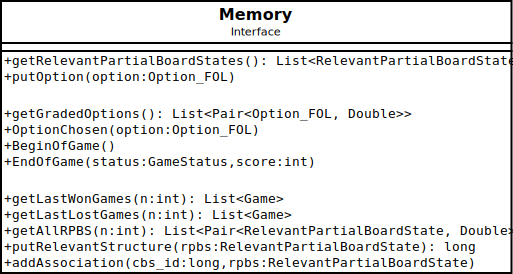
\includegraphics[width=0.9\textwidth]{img/implementation_memory/interface}
\end{center}
\end{frame}

\begin{frame}{Mémoire}{Mémoire épisodique}
\def\imgsize{\textwidth}
\only<1>{
\includegraphics[width=\imgsize]{img/implementation_memory/1_episodic_general}
}
\only<2>{
\includegraphics[width=\imgsize]{img/implementation_memory/2_episodic_general}
}
\only<3>{
\includegraphics[width=\imgsize]{img/implementation_memory/3_episodic_general}
}
\only<4>{
\includegraphics[width=\imgsize]{img/implementation_memory/4_episodic_general}
}
\only<5>{
\includegraphics[width=\imgsize]{img/implementation_memory/5_episodic_general}
}
\only<6>{
\includegraphics[width=\imgsize]{img/implementation_memory/6_episodic_general}
}
\end{frame}

\begin{frame}{Mémoire}{Mémoire sémantique}
\only<1>{
\begin{block}{Vision matricielle}
\begin{center}
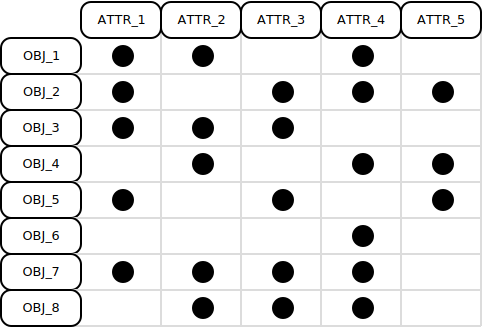
\includegraphics[width=0.6\textwidth]{img/implementation_memory/context_matrix}
\end{center}
\end{block}
}
\only<2>{
\begin{block}{Vision en graphe}
\begin{center}
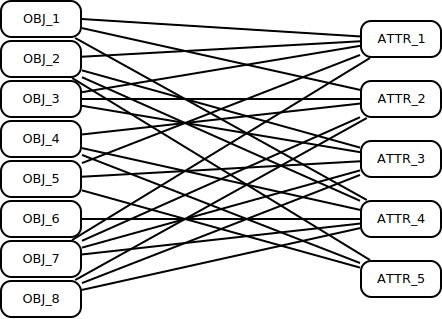
\includegraphics[width=0.6\textwidth]{img/implementation_memory/context_graph}
\end{center}
\end{block}
}
\end{frame}

\begin{frame}{Mémoire}{Persistance}
\begin{center}
\includegraphics[width=0.3\textwidth]{img/neo4j/neo4j_logo}
\end{center}
\begin{block}{Neo4j}
\begin{itemize}
\item Logiciel libre (GPLv3 / AGPLv3)
\item SGBD NoSQL orienté graphe
\item Respect des caractéristiques ACID
\item Multiple versions (embedded in Java)
\end{itemize}
\end{block}
\end{frame}

\begin{frame}{Mémoire}{Persistance}
\begin{block}{Élements}
\begin{itemize}
\item Noeud racine
\item Noeuds
\item Relations (orientées)
\item Types de relations
\item Attributs (Noeuds \& Relations)
\end{itemize}
\end{block}
\begin{block}{Comment typer les noeuds ?}
\begin{enumerate}
\uncover<2>{
\item Créer un noeud \texttt{Maitre}
\item Créer une relation typée \texttt{Racine $\rightarrow$ Maitre}
\item Créer des relations typées \texttt{Maitre $\rightarrow$ Noeuds}
}
\end{enumerate}
\end{block}

\end{frame}

\def\imgsize{0.8\textwidth}
\begin{frame}{Mémoire}{Graphe de la mémoire sémantique}
\begin{center}
\only<1>{\includegraphics[width=\imgsize]{img/neo4j/1_lattice_graph}}
\only<2>{\includegraphics[width=\imgsize]{img/neo4j/2_lattice_graph}}
\only<3>{\includegraphics[width=\imgsize]{img/neo4j/3_lattice_graph}}
\only<4>{\includegraphics[width=\imgsize]{img/neo4j/4_lattice_graph}}
\end{center}
\end{frame}

\def\imgsize{\textwidth}
\begin{frame}{Mémoire}{Graphe de la mémoire épisodique}
\begin{center}
\only<1>{\includegraphics[width=\imgsize]{img/neo4j/1_episodic_graph}}
\only<2>{\includegraphics[width=\imgsize]{img/neo4j/2_episodic_graph}}
\only<3>{\includegraphics[width=\imgsize]{img/neo4j/3_episodic_graph}}
\only<4>{\includegraphics[width=\imgsize]{img/neo4j/4_episodic_graph}}
\only<5>{\includegraphics[width=\imgsize]{img/neo4j/5_episodic_graph}}
\only<6>{\includegraphics[width=\imgsize]{img/neo4j/6_episodic_graph}}
\only<7>{\includegraphics[width=\imgsize]{img/neo4j/7_episodic_graph}}
\only<8>{\includegraphics[width=\imgsize]{img/neo4j/8_episodic_graph}}
\only<9>{\includegraphics[width=\imgsize]{img/neo4j/9_episodic_graph}}
\end{center}
\end{frame}

\begin{frame}{Mémoire}{Graphe complet de la mémoire}
\begin{center}
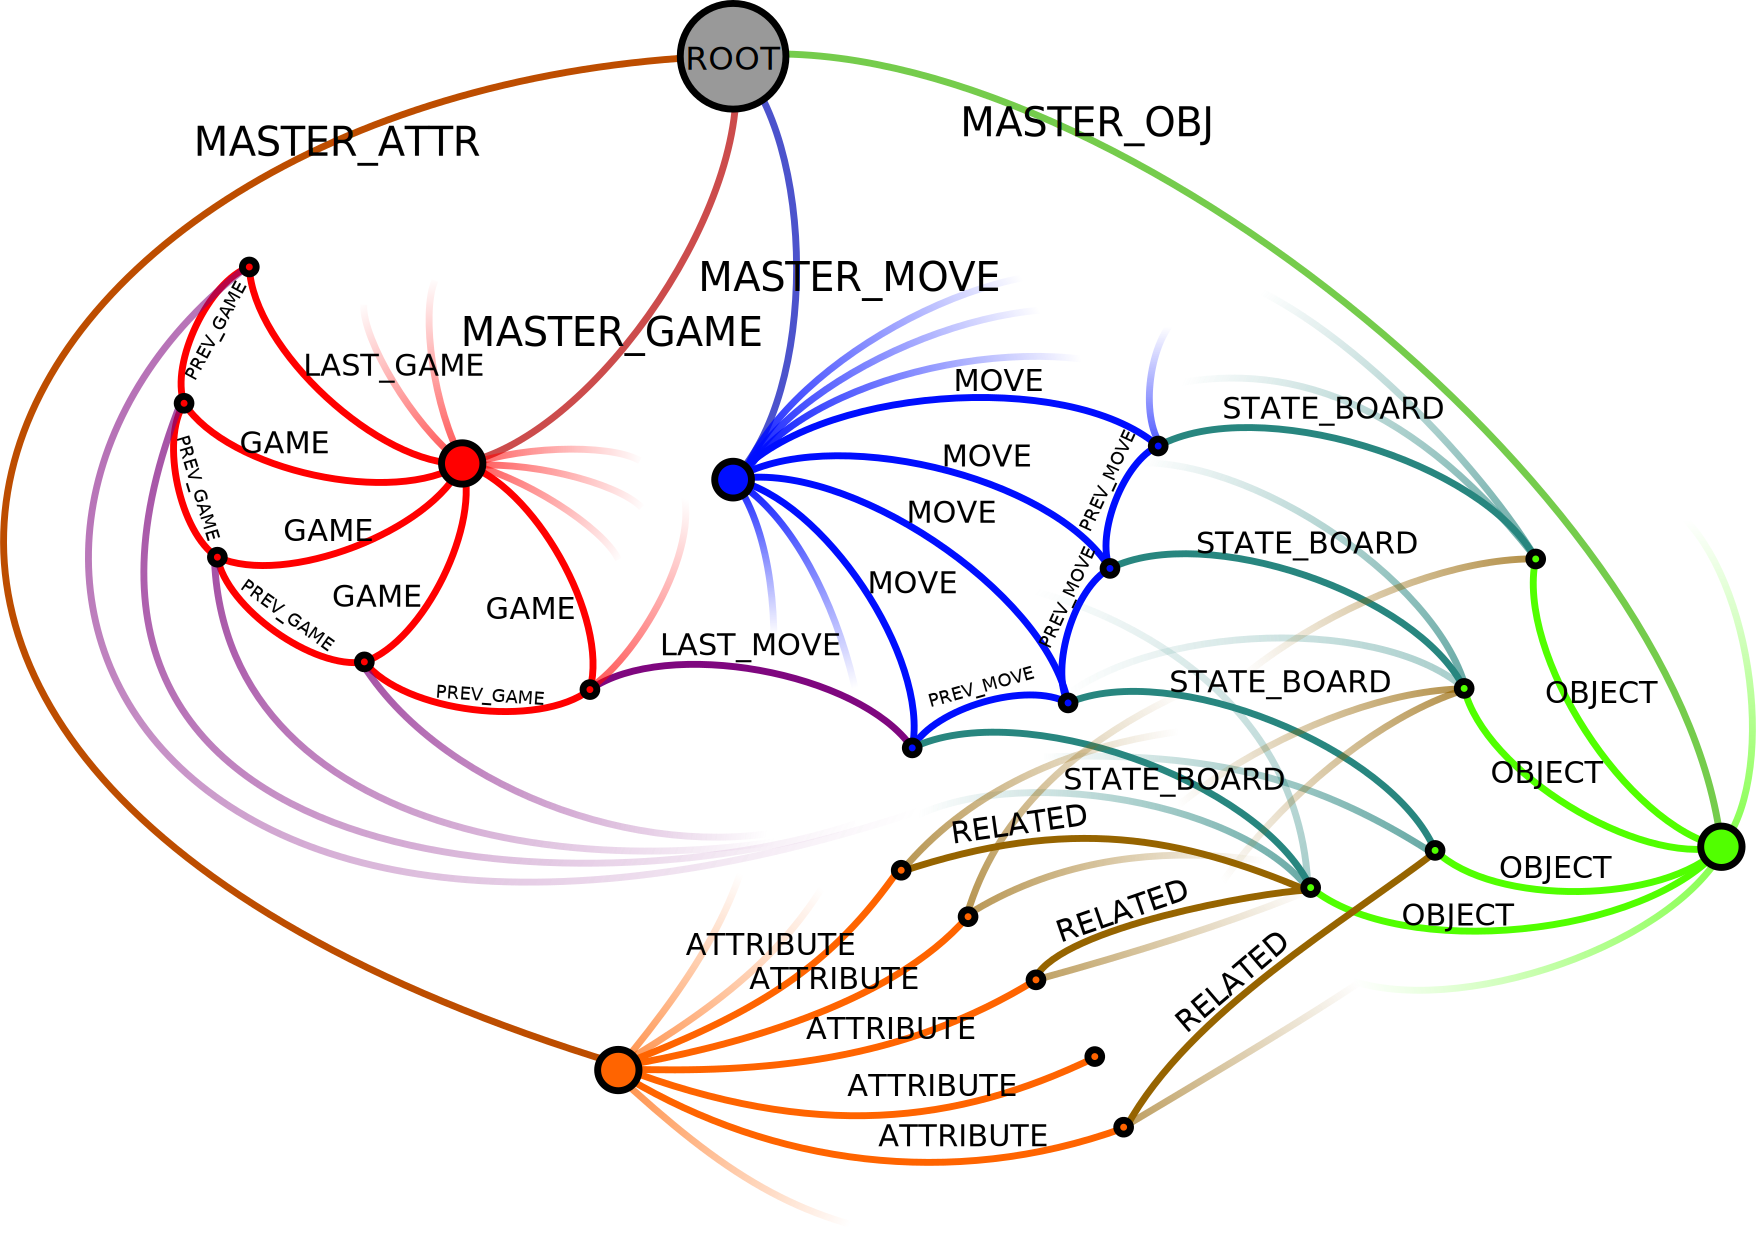
\includegraphics[width=0.8\textwidth]{img/neo4j/full_graph}
\end{center}
\end{frame}
